\documentclass{standalone}
\usepackage{tikz}
\usetikzlibrary{patterns, positioning}


\begin{document}
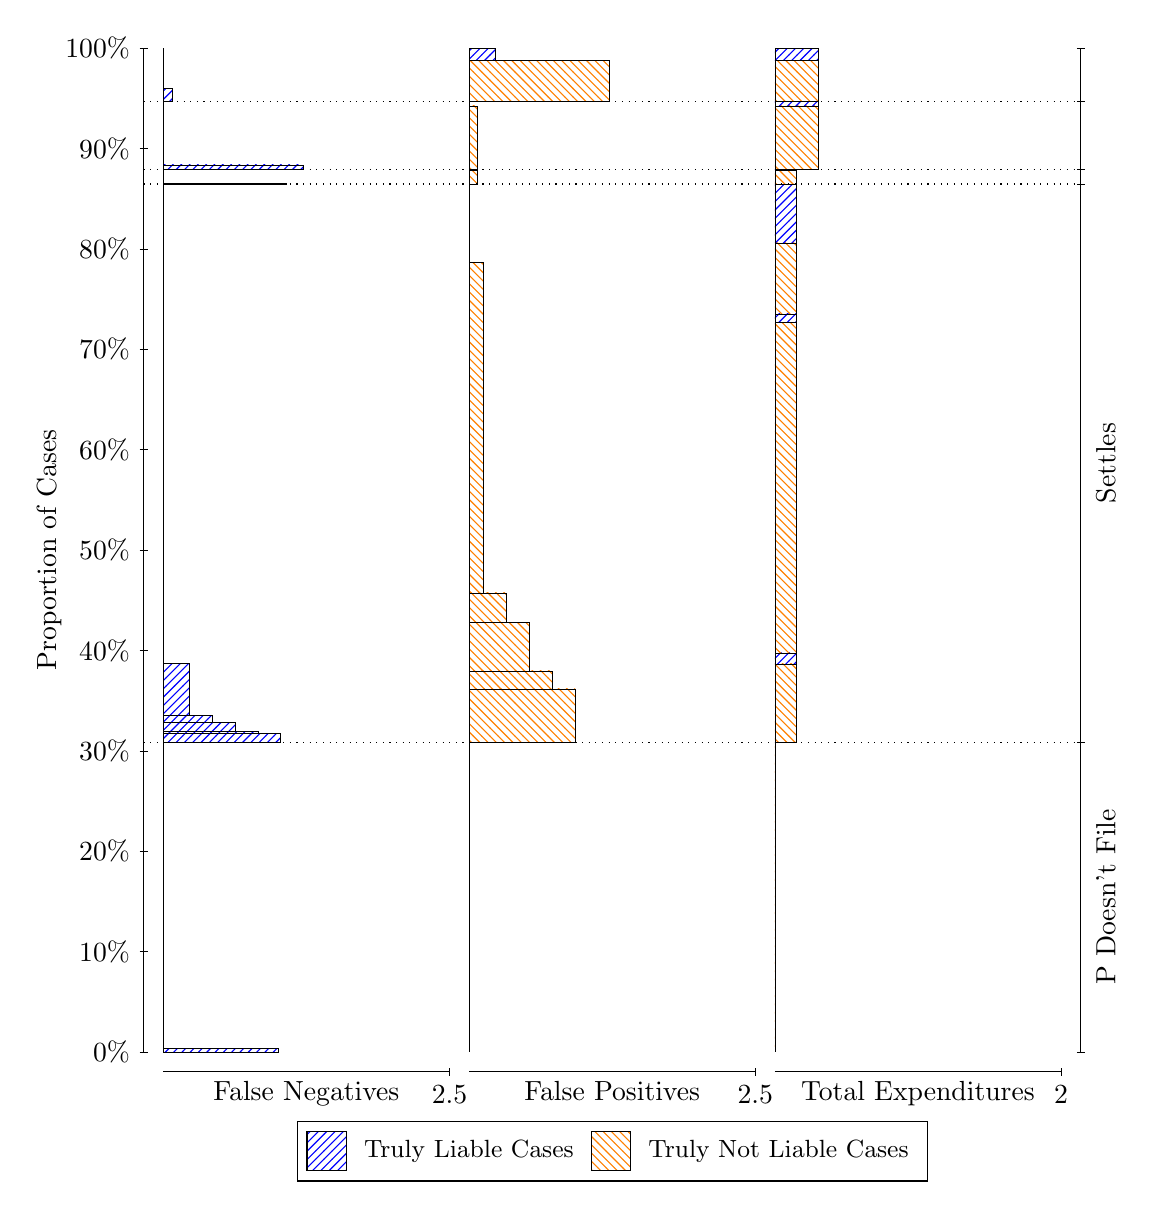
\begin{tikzpicture}
\draw[black, very thin] (1.5,1.75) -- (1.5,14.5);
\node[rotate=90, text=black, anchor=center] at (0.3, 8.125) {Proportion of Cases};
\draw[black, very thin] (1.45,1.75) -- (1.55,1.75);
\node[text=black, anchor=east] at (1.45, 1.75) {0\%};
\draw[black, very thin] (1.45,3.025) -- (1.55,3.025);
\node[text=black, anchor=east] at (1.45, 3.025) {10\%};
\draw[black, very thin] (1.45,4.3) -- (1.55,4.3);
\node[text=black, anchor=east] at (1.45, 4.3) {20\%};
\draw[black, very thin] (1.45,5.575) -- (1.55,5.575);
\node[text=black, anchor=east] at (1.45, 5.575) {30\%};
\draw[black, very thin] (1.45,6.85) -- (1.55,6.85);
\node[text=black, anchor=east] at (1.45, 6.85) {40\%};
\draw[black, very thin] (1.45,8.125) -- (1.55,8.125);
\node[text=black, anchor=east] at (1.45, 8.125) {50\%};
\draw[black, very thin] (1.45,9.4) -- (1.55,9.4);
\node[text=black, anchor=east] at (1.45, 9.4) {60\%};
\draw[black, very thin] (1.45,10.675) -- (1.55,10.675);
\node[text=black, anchor=east] at (1.45, 10.675) {70\%};
\draw[black, very thin] (1.45,11.95) -- (1.55,11.95);
\node[text=black, anchor=east] at (1.45, 11.95) {80\%};
\draw[black, very thin] (1.45,13.225) -- (1.55,13.225);
\node[text=black, anchor=east] at (1.45, 13.225) {90\%};
\draw[black, very thin] (1.45,14.5) -- (1.55,14.5);
\node[text=black, anchor=east] at (1.45, 14.5) {100\%};

\draw[black, very thin] (13.4,1.75) -- (13.4,14.5);
\draw[black, very thin] (13.35,1.75) -- (13.45,1.75);
\node[anchor=west] at (13.35, 1.75) {};
\draw[black, very thin] (13.35,5.6854) -- (13.45,5.6854);
\node[anchor=west] at (13.35, 5.6854) {};
\draw[black, very thin] (13.35,12.773) -- (13.45,12.773);
\node[anchor=west] at (13.35, 12.773) {};
\draw[black, very thin] (13.35,12.959) -- (13.45,12.959);
\node[anchor=west] at (13.35, 12.959) {};
\draw[black, very thin] (13.35,13.823) -- (13.45,13.823);
\node[anchor=west] at (13.35, 13.823) {};
\draw[black, very thin] (13.35,14.5) -- (13.45,14.5);
\node[anchor=west] at (13.35, 14.5) {};

\draw[black, very thin, pattern color=blue, pattern=north east lines] (1.75,1.75) rectangle (3.2033,1.7982);
\draw[black, very thin, pattern color=orange, pattern=north west lines] (1.75,1.7982) rectangle (1.75,5.6854);
\draw[black, very thin, pattern color=blue, pattern=north east lines] (1.75,5.6854) rectangle (3.2397,5.7946);
\draw[black, very thin, pattern color=blue, pattern=north east lines] (1.75,5.7946) rectangle (2.949,5.8243);
\draw[black, very thin, pattern color=blue, pattern=north east lines] (1.75,5.8243) rectangle (2.6583,5.9347);
\draw[black, very thin, pattern color=blue, pattern=north east lines] (1.75,5.9347) rectangle (2.3677,6.0226);
\draw[black, very thin, pattern color=blue, pattern=north east lines] (1.75,6.0226) rectangle (2.077,6.6824);
\draw[black, very thin, pattern color=orange, pattern=north west lines] (1.75,6.6824) rectangle (1.75,12.773);
\draw[black, very thin, pattern color=blue, pattern=north east lines] (1.75,12.773) rectangle (3.3123,12.785);
\draw[black, very thin, pattern color=orange, pattern=north west lines] (1.75,12.785) rectangle (1.75,12.959);
\draw[black, very thin, pattern color=blue, pattern=north east lines] (1.75,12.959) rectangle (3.5303,13.016);
\draw[black, very thin, pattern color=orange, pattern=north west lines] (1.75,13.016) rectangle (1.75,13.823);
\draw[black, very thin, pattern color=blue, pattern=north east lines] (1.75,13.823) rectangle (1.859,13.984);
\draw[black, very thin, pattern color=orange, pattern=north west lines] (1.75,13.984) rectangle (1.75,14.5);
\draw[black, very thin, pattern color=orange, pattern=north west lines] (5.6333,1.75) rectangle (5.6333,5.6372);
\draw[black, very thin, pattern color=blue, pattern=north east lines] (5.6333,5.6372) rectangle (5.6333,5.6854);
\draw[black, very thin, pattern color=orange, pattern=north west lines] (5.6333,5.6854) rectangle (6.9777,6.361);
\draw[black, very thin, pattern color=orange, pattern=north west lines] (5.6333,6.361) rectangle (6.687,6.5887);
\draw[black, very thin, pattern color=orange, pattern=north west lines] (5.6333,6.5887) rectangle (6.3963,7.206);
\draw[black, very thin, pattern color=orange, pattern=north west lines] (5.6333,7.206) rectangle (6.1057,7.5811);
\draw[black, very thin, pattern color=orange, pattern=north west lines] (5.6333,7.5811) rectangle (5.815,11.777);
\draw[black, very thin, pattern color=blue, pattern=north east lines] (5.6333,11.777) rectangle (5.6333,12.773);
\draw[black, very thin, pattern color=orange, pattern=north west lines] (5.6333,12.773) rectangle (5.7423,12.947);
\draw[black, very thin, pattern color=blue, pattern=north east lines] (5.6333,12.947) rectangle (5.6333,12.959);
\draw[black, very thin, pattern color=orange, pattern=north west lines] (5.6333,12.959) rectangle (5.7423,13.766);
\draw[black, very thin, pattern color=blue, pattern=north east lines] (5.6333,13.766) rectangle (5.6333,13.823);
\draw[black, very thin, pattern color=orange, pattern=north west lines] (5.6333,13.823) rectangle (7.4137,14.339);
\draw[black, very thin, pattern color=blue, pattern=north east lines] (5.6333,14.339) rectangle (5.9603,14.5);
\draw[black, very thin, pattern color=orange, pattern=north west lines] (9.5167,1.75) rectangle (9.5167,5.6372);
\draw[black, very thin, pattern color=blue, pattern=north east lines] (9.5167,5.6372) rectangle (9.5167,5.6854);
\draw[black, very thin, pattern color=orange, pattern=north west lines] (9.5167,5.6854) rectangle (9.7892,6.6778);
\draw[black, very thin, pattern color=blue, pattern=north east lines] (9.5167,6.6778) rectangle (9.7892,6.818);
\draw[black, very thin, pattern color=orange, pattern=north west lines] (9.5167,6.818) rectangle (9.7892,11.013);
\draw[black, very thin, pattern color=blue, pattern=north east lines] (9.5167,11.013) rectangle (9.7892,11.123);
\draw[black, very thin, pattern color=orange, pattern=north west lines] (9.5167,11.123) rectangle (9.7892,12.026);
\draw[black, very thin, pattern color=blue, pattern=north east lines] (9.5167,12.026) rectangle (9.7892,12.773);
\draw[black, very thin, pattern color=orange, pattern=north west lines] (9.5167,12.773) rectangle (9.7892,12.947);
\draw[black, very thin, pattern color=blue, pattern=north east lines] (9.5167,12.947) rectangle (9.7892,12.959);
\draw[black, very thin, pattern color=orange, pattern=north west lines] (9.5167,12.959) rectangle (10.062,13.766);
\draw[black, very thin, pattern color=blue, pattern=north east lines] (9.5167,13.766) rectangle (10.062,13.823);
\draw[black, very thin, pattern color=orange, pattern=north west lines] (9.5167,13.823) rectangle (10.062,14.339);
\draw[black, very thin, pattern color=blue, pattern=north east lines] (9.5167,14.339) rectangle (10.062,14.5);
\draw[black, dotted] (1.5,5.6854) -- (13.4,5.6854);
\draw[black, dotted] (1.5,12.773) -- (13.4,12.773);
\draw[black, dotted] (1.5,12.959) -- (13.4,12.959);
\draw[black, dotted] (1.5,13.823) -- (13.4,13.823);
\draw[black, very thin] (1.75,1.5) -- (5.3833,1.5);
\node[text=black, anchor=north] at (3.5667, 1.5) {False Negatives};
\draw[black, very thin] (5.3833,1.45) -- (5.3833,1.55);
\node[text=black, anchor=north] at (5.3833, 1.45) {2.5};

\draw[black, very thin] (5.6333,1.5) -- (9.2667,1.5);
\node[text=black, anchor=north] at (7.45, 1.5) {False Positives};
\draw[black, very thin] (9.2667,1.45) -- (9.2667,1.55);
\node[text=black, anchor=north] at (9.2667, 1.45) {2.5};

\draw[black, very thin] (9.5167,1.5) -- (13.15,1.5);
\node[text=black, anchor=north] at (11.333, 1.5) {Total Expenditures};
\draw[black, very thin] (13.15,1.45) -- (13.15,1.55);
\node[text=black, anchor=north] at (13.15, 1.45) {2};

\node[text=black, centered, rotate=90] at (13.72, 3.7177) {P Doesn't File};
\node[text=black, centered, rotate=90] at (13.72, 9.2295) {Settles};




\draw (7.449999999999999,1.5) node[draw=none] (baseCoordinate) {};
\begin{scope}[align=center]
        \matrix[scale=0.5, draw=black, below=0.5cm of baseCoordinate, nodes={draw}, column sep=0.1cm]{
            \node[rectangle, draw, minimum width=0.5cm, minimum height=0.5cm, pattern color=blue, pattern=north east lines] {}; &
            \node[draw=none, font=\small, text=black] (B) {Truly Liable Cases}; &
            \node[rectangle, draw, minimum width=0.5cm, minimum height=0.5cm, pattern color=orange, pattern=north west lines] {}; &
            \node[draw=none, font=\small, text=black] (B) {Truly Not Liable Cases}; \\
            };
\end{scope}

\end{tikzpicture}
\end{document}